\chapter{Układ zamka}
\label{chap:controller}

    Niniejszy rozdział przedstawia zagadnienia związane z procesem implementacji układu zamka. Uzasadnia wybór wykorzystanych w projekcie technologii sprzętowych i programowych, opisuje sposób konfiguracji środowiska deweloperskiego, a także przedstawia wybrane problemy implementacyjne.

    \section{Wykorzystane technologie}

        \subsection{Mikrokontroler}

            Istotnym problemem natury implementacyjnej jest wybór odpowiedniego mikrokontrolera, który spełni wymagania dotyczące wydajności energetycznej oraz bezpieczeństwa systemu, jednocześnie zapewniając możliwość obsługi kilku układów peryferyjnych i wsparcie dla komunikacji bezprzewodowej, a także wygodne i elastyczne środowisko deweloperskie.

            Spośród wielu rozwiązań dostępnych na rynku wybrany został mikrokontroler ESP32. Oprócz wszystkich wymienionych wyżej cech, charakteryzuje się on możliwością przetwarzania równoległego za pomocą dwóch fizycznych rdzeni, co otwiera nowe możliwości w kwestii projektowania i implementacji oprogramowania, szczególnie w przypadku istnienia rygorystycznych wymagań dotyczących czasu odpowiedzi układu. Zapewnia sprzętowe wsparcie dla algorytmów kryptograficznych oraz możliwość zaawansowanej kontroli pracy podzespołów w zakresie zasilania, a także umożliwia komunikację z peryferiami za pośrednictwem programowalnych wejść/wyjść GPIO (ang. \textit{General-Purpose Input/Output}).

            Oprogramowanie dla mikrokontrolera ESP32 może być wytwarzane w środowisku Arduino IDE lub z wykorzystaniem oficjalnej platformy programistycznej Espressif IoT Development Framework (ESP-IDF) firmy Espressif Systems. ESP-IDF opiera się na systemie FreeRTOS (ang. \textit{Free Real-Time Operating System}, system operacyjny czasu rzeczywistego), w wersji 8.2.0, port Xtensa~\cite{esp-idf-freertos-smp-changes}. Ze względu na chęć uzyskania pełniejszej kontroli nad mikrokontrolerem zdecydowano się na użycie w projekcie platformy ESP-IDF.

        \subsection{Czytnik RFID}

            Głównym kryterium wyboru czytnika identyfikatorów RFID jest prostota integracji z mikrokontrolerem. Ze względu na fakt, iż jego zasilaniem zarządzać będzie mikrokontroler, niski pobór mocy nie stanowi kryterium przesądzającego. Wybrano układ MFRC522 produkowany przez firmę NXP Semiconductors. Układ obsługuje urządzenia o częstotliwości nośnej 13,56 MHz oraz umożliwia komunikację poprzez protokół SPI (ang. \textit{Serial Peripheral Interface}).

        \subsection{Czujnik ruchu}

            Czujnik ruchu posiada krytyczne znaczenie w układzie zamka. Jako jedyny z podzespołów musi być zasilany przez cały czas pracy układu. Ze względu na wymaganie wykorzystania zasilania bateryjnego w układzie istotną cechą jest jak najniższy pobór mocy w stanie spoczynku. Wybranym rozwiązaniem jest czujnik PIR (ang. \textit{Passive Infrared}, pasywny czujnik podczerwieni), model HC-SR501. Wykrycie obiektu sygnalizowane jest stanem wysokim na cyfrowym wyjściu, natomiast maksymalny zasięg wykrywania wynosi 3-7 m. Czujnik wyposażony jest w dwa potencjometry umożliwiające regulację czasu trwania stanu wysokiego po wykryciu obiektu oraz czułości czujnika. Układ posiada także zworkę, za pomocą której można wybrać jeden z dwóch możliwych trybów:

            \begin{itemize}
                \item Tryb \textit{retriggering} - po wykryciu obiektu stan wysoki utrzymywany jest przez określony przez potencjometr czas,
                \item Tryb \textit{non-retriggering} - stan wysoki po wykryciu obiektu utrzymywany jest przez cały czas występowania ruchu. Po zatrzymaniu ruchu stan wysoki utrzymywany jest przez określony przez potencjometr czas.
            \end{itemize}

            Dzięki temu możliwe jest dobranie parametrów czujnika w taki sposób, aby użytkownik był wykrywany w odpowiednim momencie, co przekłada się na bardziej optymalne działanie układu.

            Aby zapewnić wykrycie zbliżającego się użytkownika w optymalnym dla pracy układu czasie, poziom czułości czujnika został ustawiony na wartość minimalną 3 m. Długość czasu trwania stanu wysokiego po wykryciu obiektu została ustawiona na wartość minimalną celem uzyskania impulsu stanowiącego źródło wybudzenia mikrokontrolera. Wybrany został tryb \textit{retriggering} w celu zapewnienia poprawnego działania układu w sytuacji gdy użytkownik zostanie wykryty, lecz nie zdąży przyłożyć identyfikatora do czytnika w zadanym okresie czasu. Dzięki zastosowaniu trybu \textit{retriggering} możliwe jest ponowne wykrycie użytkownika po jego zbliżeniu się do zamka.

            \textbf{TBD - schemat jak sa polaczone pinami te wszystkie komponenty}

        \subsection{Połączenia komponentów}

            Rysunek \ref{fig:lock_hardware_schematic} przedstawia sposób połączenia komponentów sprzętowych. Układ HC-SR501 komunikuje się z mikrokontrolerem umieszczonym na płytce ESP32-DevKitC-32D przez pojedynczą linię sygnałową. Czytnik MFRC522 w celu komunikacji z mikrokontrolerem wykorzystuje interfejs SPI. Głównym źródłem zasilania jest źródło stałoprądowe o napięciu w granicach 5~V. Jest ono wykorzystywane bezpośrednio przez układ mikrokontrolera i czujnika ruchu. Platforma ESP32-DevKitC-32D zapewnia dodatkowo źródło zasilania napięciem o wartości 3,3~V. które za pośrednictwem układu sterującego wykorzystywane jest do zasilania czytnika.

            \begin{figure}[]
                \centering
                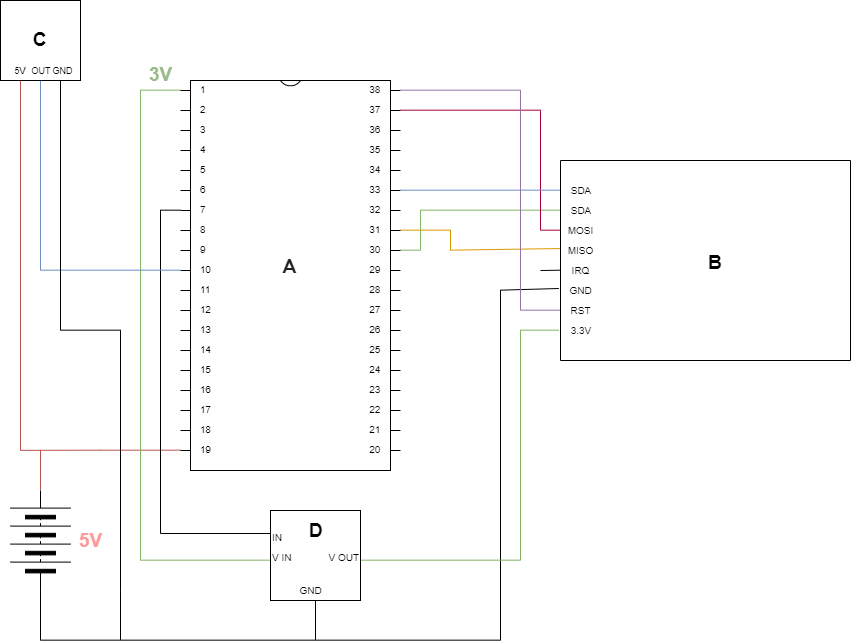
\includegraphics[width=\textwidth]{chapters/images/lock_hardware_schematic.png}
                \caption[Schemat połączeń w układzie zamka] {
                    Schemat połączeń w układzie zamka.
                    \textbf{(A)} ESP32-DevKitC-32D
                    \textbf{(B)} Czytnik MFRC522
                    \textbf{(C)} Czujnik ruchu HC-SR501
                    \textbf{(D)} Układ sterujący zasilaniem czytnika
                }
                \label{fig:lock_hardware_schematic}
            \end{figure}

        \subsection{Układ sterujący zasilaniem czytnika RFID}

            Układ czytnika wymaga zasilania napięciem 3,3V o mocy do 330mW~\cite{mfrc522-ds}. Jest to kosztowne z punktu widzenia wydajności energetycznej, dlatego z chwilą wprowadzenia mikrokontrolera w stan głębokiego uśpienia czytnik musi zostać wyłączony. Wyjścia mikrokontrolera są łatwo dostępnym i kontrolowanym programowo źródłem napięcia, jednak ze względu na niską wydajność prądową, nie można ich wykorzystać do bezpośredniego zasilania układów o mocy powyżej 130mW~\cite{esp32-ds}. Dlatego zastosowano przedstawiony na rysunku \ref{fig:rfid_power_relay} układ przełączający. Stan wysoki na wejściu układu otwiera kanał tranzystora przełączającego co umożliwia przepływ prądu przez układ i w efekcie zasilenie układu czujnika.

            \begin{figure}[]
                \centering
                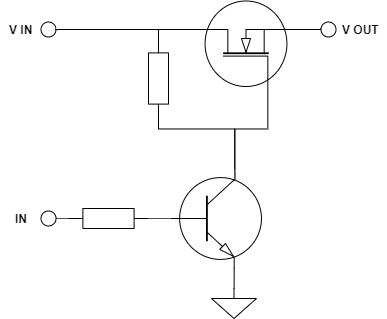
\includegraphics[width=0.5\textwidth]{chapters/images/rfid_power_relay.png}
                \caption{Schemat układu sterującego zasilaniem czytnika}
                \label{fig:rfid_power_relay}
            \end{figure}



    \section{Konfiguracja środowiska}

        Platforma programistyczna ESP-IDF zapewnia zestaw narzędzi (ang. \textit{toolchain}) umożliwiających wytwarzanie oprogramowania dla mikrokontrolera ESP32. Platforma ESP-IDF dostępna jest jako projekt otwartoźródłowy na licencji Apache 2.0 w serwisie github.

        Komponenty potrzebne do wytwarzania oprogramowania dla ESP32 z użyciem ESP-IDF oraz sam proces w uproszczeniu przedstawia rysunek \ref{fig:esp32_dev} \cite{esp-idf-get-started}.

        \begin{figure}[]
            \centering
            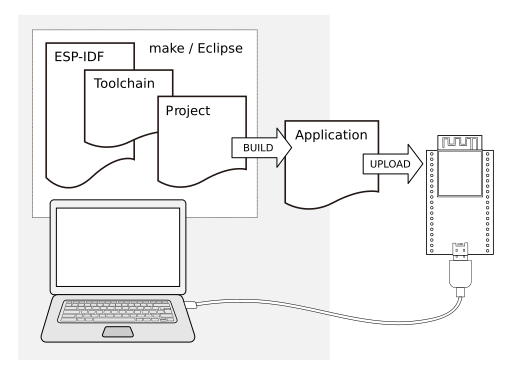
\includegraphics[width=\textwidth]{chapters/images/esp32_dev.png}
            \caption{Wytwarzanie oprogramowania dla ESP32}
            \label{fig:esp32_dev}
        \end{figure}

        Konfiguracja, budowanie aplikacji i programowanie mikrokontrolera odbywa się za pomocą dedykowanego skryptu dostarczanego przez platformę.

    \section{Oprogramowanie mikrokontrolera}

        \subsection{Komponenty}

            ESP-IDF umożliwia podział aplikacji na komponenty oraz ich łatwą konfigurację w procesie kompilacji za pomocą tekstowego menu (tzw. \textit{menuconfig}). Jak wyjaśnia \cite{esp-idf-build-system}, komponenty to modularne i samodzielne fragmenty kodu kompilowane do bibliotek statycznych i dołączane do aplikacji. Niektóre z nich są dostarczane przez platformę ESP-IDF. Istnieje też możliwość tworzenia własnych komponentów.

            Kod źródłowy oprogramowania mikrokontrolera został podzielony na następujące komponenty:

            \begin{enumerate}
                \item Komponent główny (\texttt{main})

                    Odpowiedzialny za inicjalizację niezbędnych modułów i przejście w tryb głębokiego uśpienia w przypadku standardowego uruchomienia mikrokontrolera. W przypadku zdarzenia wybudzenia z głębokiego uśpienia odpowiedzialny dodatkowo za wywołanie kodu należącego do komponentu sterującego. Składa się z pojedynczego pliku źródłowego.

                \item Komponent RFID

                    Odpowiedzialny za komunikację z czytnikiem RFID. Składa się z zewnętrznej biblioteki obsługującej czytnik MFRC522 (patrz \ref{sub:rfid_lib}), pliku ze zbiorem funkcji umożliwiających jej łatwą obsługę oraz pliku z funkcjami związanymi z zadaniem \texttt{rfid} (patrz \ref{sub:tasks}).

                \item Komponent WiFi

                    Odpowiedzialny za nawiązanie połączenia z siecią bezprzewodową i serwerem oraz przeprowadzenie procesu wymiany informacji w celu autoryzacji identyfikatora. Składa się z biblioteki obsługującej komunikację za pomocą socket'ów, biblioteki obsługującej komunikację z wykorzystaniem protokołu TLS (patrz \ref{sub:tls}), kilku plików z funkcjami pomocniczymi oraz pliku z funkcjami związanymi z zadaniem \texttt{wifi}. To, czy komunikacja z serwerem odbywać się będzie z wykorzystaniem TLS, definiowane jest przez opcję \texttt{TLS\_ENABLED} zawartą w opcjach \textit{menuconfig} komponentu WiFi.

                \item Komponent GPIO

                    Odpowiedzialny za obsługę komunikacji za pomocą GPIO w celu kontroli zasilania czytnika MFRC522. Składa się z pojedynczego pliku zawierającego proste funkcje umożliwiające ustawianie żądanych stanów na wyjściach.

                \item Komponent sterujący (\textit{flow-controller})

                    Odpowiedzialny za wykonanie i nadzór nad przepływem sterowania od momentu wybudzenia z głębokiego uśpienia aż do zakończenia procesu komunikacji z serwerem. Składa się z pliku zawierającego funkcję obsługującą cały proces oraz pliku definiującego mechanizm synchronizacji zadań (patrz \ref{sub:tasks}).

            \end{enumerate}

            Szczegółowy opis struktury kodu umieszczono w dodatku \ref{app:app1}.

        \subsection{Współbieżność}
        \label{sub:tasks}

            Jak opisuje \cite{esp-idf-freertos-smp-changes}, oryginalny system FreeRTOS został zaprojektowany z myślą o przetwarzaniu za pomocą jednego rdzenia. ESP32 posiada jednak dwa rdzenie o wspólnej pamięci, co pozwala na przemienne wykonywanie zadań na obu rdzeniach. Koncepcja zadań (ang. \textit{tasks}) istniejąca w oryginalnym systemie FreeRTOS w ESP-IDF została zmodyfikowana na potrzeby wsparcia mikrokontrolera o dwóch rdzeniach oraz SMP (ang. \textit{symmetric multiprocessing}, symetryczne przetwarzanie wieloprocesorowe). Każde z zadań ma określony priorytet, na podstawie którego algorytm planowania ustala kolejność wykonywania. Dzieje się to indywidualnie dla każdego rdzenia, lecz lista zadań gotowych do wykonania jest pomiędzy nimi współdzielona.

            Aby maksymalnie wykorzystać możliwości platformy ESP-IDF w kwestii współbieżności jednocześnie unikając nadmiernego skompilowania kodu, zdecydowano się na wykorzystanie w ramach aplikacji dwóch zadań. Należy nadmienić, że mikrokontroler przez większą część czasu wykonuje operacje, których zrównoleglenie nie przyniosłoby korzyści. Jedyną sytuacją, w której warto zastosować przetwarzanie współbieżne jest nawiązywanie połączenia z serwerem oraz odczyt danych z czytnika RFID. Obie czynności mogą okazać się czasochłonne. W aplikacji jednowątkowej, odczyt danych z czytnika RFID musiałby zakończyć się przed rozpoczęciem nawiązywania połączenia, lub odwrotnie. Jeśli zostanie zastosowany zapewniany przez ESP-IDF mechanizm zadań, możemy wykonywać obie operacje jednocześnie. Zdefiniowano zatem następujące zadania:

            \begin{enumerate}
                \item Zadanie \texttt{wifi},
                \item Zadanie \texttt{rfid}.
            \end{enumerate}

            Do synchronizacji zadań wykorzystany został mechanizm tzw. \textit{event group} (grupy zdarzeń) dostarczany przez system FreeRTOS. Zakłada on wykorzystanie przez współpracujące zadania współdzielonej grupy zdarzeń, składającej się z zestawu flag, oraz udostępnia funkcje do operowania na niej. Możliwe operacje to ustawianie w stan wysoki lub niski danej flagi oraz oczekiwanie na stan wysoki flagi. Korzystny z perspektywy synchronizacji wątków jest fakt, że oczekiwanie na dane zdarzenie blokuje aktualnie wykonywane zadanie, umożliwiając oddanie sterowania innym oczekującym zadaniom.

        \subsection{Stan głębokiego uśpienia}

            ESP32 oferuje efektywną i elastyczną technologię zarządzania energią. Dokument \cite{esp32-ds} wymienia pięć dostępnych stanów energetycznych:

            \begin{enumerate}
                \item Tryb aktywny (\textit{Active mode})

                    Aktywne CPU wraz z układem radiowym.

                \item Tryb z uśpionym modemem (\textit{Modem-sleep mode})

                    Aktywne CPU, układ radiowy wyłączony.

                \item Tryb lekkiego uśpienia (\textit{Light-sleep mode})

                    Uśpione CPU. Pamięć i peryferia RTC (ang. \textit{Real-Time Clock}, zegar czasu rzeczywistego) wraz z koprocesorem ULP (ang. \textit{Ultra Low Power co-processor}) są aktywne. Jakiekolwiek zdarzenia wybudzające doprowadzą do wybudzenia układu.

                \item Tryb głębokiego uśpienia (\textit{Deep-sleep mode})

                    Tylko pamięć i peryferia RTC pozostają zasilone. Dane dotyczące połączeń WiFi i Bluetooth zostają przechowane w pamięci RTC. Opcjonalnie dostępny jest koprocesor ULP.

                \item Tryb hibernacji (\textit{Hibernation mode})

                    Wewnętrzny rezonator kwarcowy wraz z koprocesorem ULP zostają wyłączone. Również pamięć RTC jest wyłączona. Wybudzenie możliwe jest tylko poprzez regulator czasowy RTC (ang. \textit{RTC timer}) lub wejścia RTC GPIO.

            \end{enumerate}

            \textbf{Można dodać jakie są zużycia energii tutaj}

            Z punktu widzenia wymagań dotyczących poboru energii niezwykle przydatnym trybem jest tryb głębokiego uśpienia (ang. \textit{deep-sleep mode}). Dzięki jego wykorzystaniu możliwe jest przebywanie mikrokontrolera w trybie niskiego zużycia energii przez większą część czasu. Ze względu na cyfrowy charakter wyjścia czujnika ruchu, jako sposób wybudzenia mikrokontrolera skonfigurowano tryb EXT0 (ang. \textit{External Wakeup 0}, wybudzenie zewnętrzne) umożliwiający wykorzystanie modułu RTC IO (ang. \textit{Real-Time Clock Input Output}) w celu zainicjowania wybudzenia. Inne możliwe źródła wybudzenia to m.in. regulator czasowy RTC czy przerwanie wbudowanego czujnika dotykowego (ang. \textit{touch pad}). Konfiguracja trybu wybudzania odbywa się programowo.

        \subsection{Biblioteka do zarządzania czytnikiem RFID}
        \label{sub:rfid_lib}

            Do zarządzania czytnikiem MFRC522 wykorzystano zewnętrzną bibliotekę\footnote{Alija Bobija, \textit{C library for interfacing ESP32 with MFRC522 RFID card reader}, \url{https://github.com/abobija/esp-idf-rc522} (rewizja 557af67)}.

        \subsection{Komunikacja z wykorzystaniem TLS}
        \label{sub:tls}

            TLS (ang. \textit{Transport Layer Security}) jest rozwinięciem protokołu SSL (ang. \textit{Secure Socket Layer}). TLS zapewnia poufność oraz integralność transmisji. Umożliwia też uwierzytelnienie serwera, a czasami również klienta.
            Protokół TLS w wersji 1.3 zaproponowano w dokumencie \cite{rfc8446}. Dokument definiuje podprotokół uścisku dłoni (ang. \textit{handshake}), dzięki któremu klient i serwer mogą uzgodnić wersję protokołu, rodzaj używanych algorytmów kryptograficznych, opcjonalnie dokonać wzajemnego uwierzytelnienia, a także ustanowić klucze kryptograficzne. Po dokonaniu uścisku dłoni, strony używają ustalonych kluczy celem zabezpieczenia przesyłanych danych.
            \textit{Handshake} TLS składa się z trzech faz:

            \begin{itemize}

                \item Wymiana kluczy

                    Ustalenie kluczy oraz wybór parametrów kryptograficznych. Od tego momentu wymieniane dane są zaszyfrowane.

                \item Parametry serwera

                    Uzgodnienie pozostałych parametrów uścisku dłoni (np. konieczność uwierzytelnienia klienta).

                \item Uwierzytelnienie

                    Uwierzytelnienie serwera i opcjonalnie klienta.
            \end{itemize}

            ESP-IDF umożliwia korzystanie z komponentu ESP-TLS, który zapewnia prosty interfejs dla najczęściej wykorzystywanych funkcjonalności protokołu TLS. Jako bazowa biblioteka tego komponentu używana jest biblioteka mbedTLS.

            Dzięki możliwości osadzenia plików binarnych w definicji komponentu zapewnianej przez ESP-IDF łatwym staje się dołączenie do oprogramowania niezbędnych certyfikatów.

            Certyfikaty zostały wygenerowane za pomocą biblioteki OpenSSL. Pierwszym krokiem było wygenerowanie certyfikatu CA (ang. \textit{Certificate Authority}, urząd certyfikacji). Następnie wygenerowano klucze prywatne oraz certyfikaty dla klienta (mikrokontrolera) oraz serwera.

            Z punktu widzenia bezpieczeństwa systemu korzystnym jest uwierzytelnienie zarówno serwera, jak i klienta. Mechanizm taki został zaimplementowany w systemie poprzez odpowiednią konfigurację oprogramowania serwera autoryzacji (patrz \ref{s:auth_subs}).

        \subsection{Przepływ sterowania}

            Przepływ sterowania w oprogramowaniu mikrokontrolera ukazują rysunki \ref{fig:flowchart1} i \ref{fig:flowchart4}. Na rysunkach \ref{fig:flowchart2} i \ref{fig:flowchart3} przedstawiono przepływ sterowania w zadaniach \textit{wifi} i \textit{rfid}.

            \begin{figure}[]
                \centering
                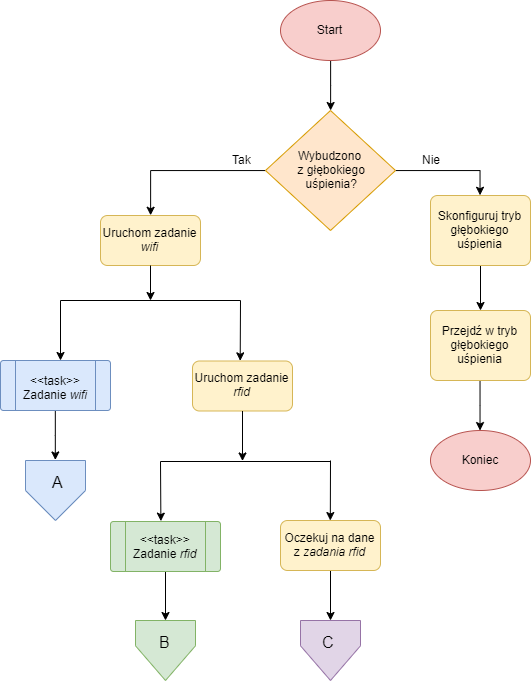
\includegraphics[width=\textwidth]{chapters/images/flowchart1.png}
                \caption{Schemat blokowy przepływu sterowania oprogramowania mikrokontrolera}
                \label{fig:flowchart1}
            \end{figure}

            \begin{figure}[]
                \centering
                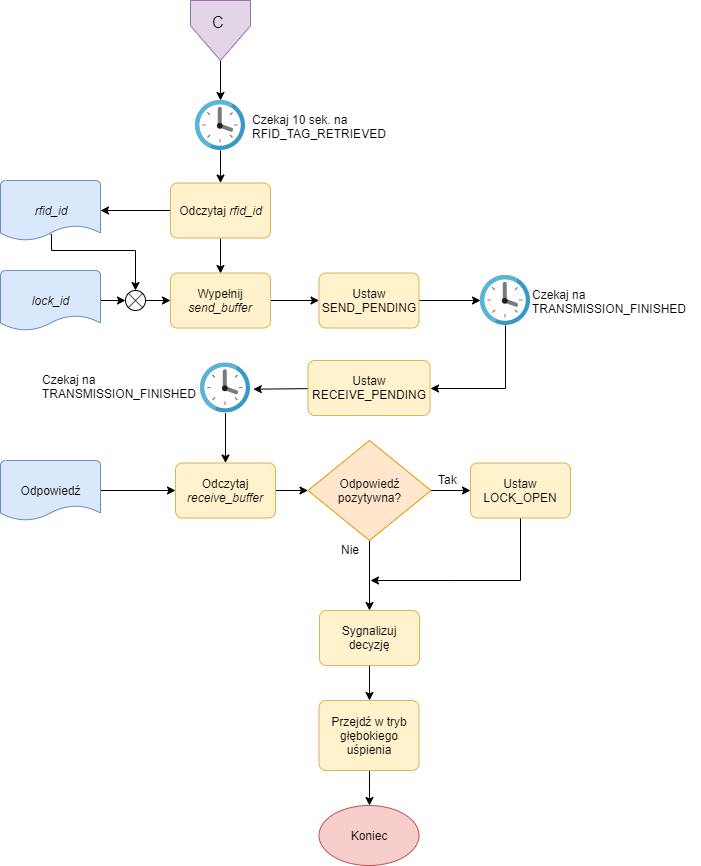
\includegraphics[width=\textwidth]{chapters/images/flowchart4.png}
                \caption{Schemat blokowy przepływu sterowania oprogramowania mikrokontrolera, c.d.}
                \label{fig:flowchart4}
            \end{figure}

            \begin{figure}[]
                \centering
                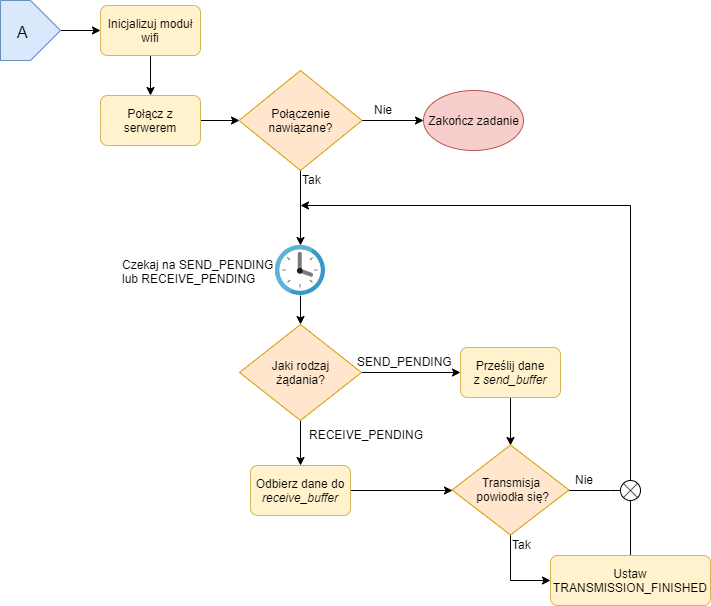
\includegraphics[width=\textwidth]{chapters/images/flowchart2.png}
                \caption{Schemat blokowy przepływu sterowania zadania obsługującego komunikację z serwerem}
                \label{fig:flowchart2}
            \end{figure}

            \begin{figure}[]
                \centering
                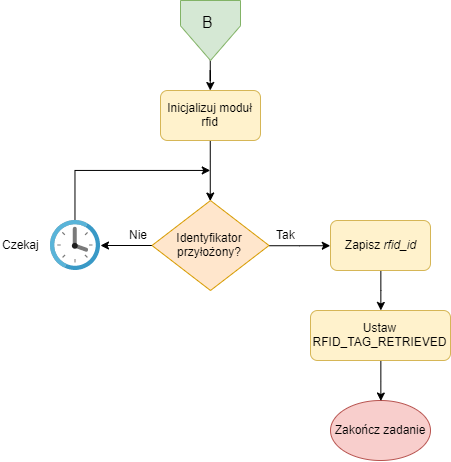
\includegraphics[width=0.8\textwidth]{chapters/images/flowchart3.png}
                \caption{Schemat blokowy przepływu sterowania zadania obsługującego czytnik RFID}
                \label{fig:flowchart3}
            \end{figure}